\section{Representations in Design-by-Analogy} %数字是飞书-论文筛选-论文归类sheet1的序号
We refer to previous work\cite{hertzmann2023image, linsey2008modality}, articles related to the analogy theory\cite{gentner1983structure}, and the corpus collection, we obtain the following forms of representation.
%我们参考以往工作和analogy理论相关文章基于语料库收集得到如下表现形式。

%语义/文字
\textbf{\underline{Semantics and text.}} It refers to make analogy at the concepts and contextual semantic levels. This can be stratified into several tiers: The first level is using textual analogies for identifying similarity, leveraging narrative analogies in personalized writing and crowdsourced creative writing ideation. For instance, Shao et al. and Ju
et al. employ analogy generation at the sentence/phrase level to produce empathetic stories and comprehensible scientific instructional content \cite{shao2025unlock, Ju2025toward}. Srinivasan et al. and Yu et al. utilize crowdsourced ideation, chunking, and recombination to generate novel far-domain analogical inspirations or innovative design concepts\cite{srinivasan2024improving, yu2014distributed}. The second level is using lingustic concepts as the domain transfer mediation, for instance, Researchers respectively achieve cross-disciplinary, cross-manufacturing-process, and cross-modal conceptual mapping through retrieval of relevant knowledge\cite{zheng2024disciplink, emerson2024anther, chen2024BIDTrain, yan2023xcreation} . And works compile domain knowledge into text-centric repositories for function tracking and context mapping in geotechnical engineering, service design, data products, and military systems \cite{you2018design, moreno2014analogies, chen2024beyond, yucelmics2018procedure}.

%语义和文字的定义是在概念和上下文语义上进行类比。分为几个层次,第一个层次是使用文字类比来识别相似性,在个性化写作和众包创意写作构思中利用叙事类比。如【49】【44】工作利用类比法生成语句字段级别的类比,产出令人产生同理心的故事和令人理解的科学教学内容;【1】【5】工作使用众包创意、组块和重组等方法生成新的远域类比灵感或者新的设计概念和构思。第二个层次是使用语言概念作为领域转移的中介,例如,【13】【3】【7】【15】分别是通过检索相关的知识,完成跨学科的,跨制造工艺,跨模态的概念映射;【72】【76】【10】【60】将领域知识总结为文字为主的知识库用于岩土工程、服务设计、数据产品、军事产品的功能追踪、情境映射等。


%仅外观/形状
\textbf{\underline{Visual and Appearance.}} It refers to make visual analogies of lines, colors, style, etc. at the appearance level. 
The fundamental type is elementary visual similarity for aesthetic forms, where works such as Warner et al. employ geometric shape correspondences to achieve vector graphic style transfer\cite{warner2023interactive}, Lin et al. investigate sketch migration\cite{lin2025inkspire}, and Fischer et al.'s 3D model based analogies\cite{fischer2024nerf}. There are still some tasks based on visual concepts generalization, with \cite{yu2016distributed, edwards2024advise} dedicated to mining and generating design concepts grounded in visual resemblance. The second type is visual context relationship mapping, where Akula et al. focuses on interpreting and generating visual metaphors through semantic relations among pictorial elements\cite{akula2023metaclue}, whereas Bitton et al. addresses context-aware visual scene understanding and synthesis\cite{bitton2023vasr}. The third type is cross-domain structural remapping, as implemented in Gong et al.'s work remaps faces from creatures/films to specific faces via structured mapping\cite{gong2023toontalker}, while Peyre et al. detects and generates visual relational similarities (e.g., actions, semantics, behaviors) overlooked by conventional approaches\cite{peyre2019detecting}.

%在外观层面进行线条、色彩、风格等视觉上的类比,分为几个层次:第一个层次是使用视觉元素的相似性类比生成艺术设计作品,如【9】【50】【20】工作通过几何形状相似性生成矢量图形的样式迁移,草图的迁移以及模型相似性上的类比,还有一些工作【36】【35】致力于挖掘或生成基于视觉相似性的设计概念上的类比;【25】关注画面元素之间的语义关系,进行视觉隐喻的映射的理解与生成,而【18】工作关注并致力于理解和生成基于情境感知的视觉画面;而【27】这份工作基于结构化映射将人脸从别的生物和影片中跨域重演到特定人脸上,【26】工作致力于检测并生成传统方法忽略了的动作、语义、行为上的视觉关系相似性图片。



%材质/结构
%在材料、结构上进行类比
\textbf{\underline{Material and Structure}}. It refers to make analogical mapping at the material physical properties and structural levels. Here we categorized as follows: First, works achieve cross-domain migration through the similarities of physical properties such as material, finishing, strength, thermal conductivity, ductility, etc. For example, in product design, Fischer et al. and Khosravani
et al.'s work perform material and finishing migration according to the knowledge bases\cite{fischer2024nerf, khosravani2022intelligent}. Thomas et al. mapped mechanical fatigue characteristics to the visualizations of the factory monitoring systems\cite{thomas2013extending}. Hong et al. converting biological tissue elastic modulus to wearable flexible electronics\cite{hong2024fishbone}. Moreover, An et al. mapped the manufacturing process of wooden frame components and the experience of automated manufacturing onto new frame throught Computer Numerical Control(CNC) Machine Tool\cite{an2020bim}.
Secondly, microstructural analogy based on geometric topology (lattice, porosity, fiber arrangement): Fan et al. leverage fractal design analogies with stretchable electronic structures\cite{fan2014fractal}. Jin et al. using buckling-guided Assembly principles mapping 2D patterns to 3D structures\cite{jin2023deep}. Yu et al. investigate structural mapping of cephalopod chromatophore mechanisms to triple-layer color-changing materials\cite{yu2014adaptive}.

% %在材料物理属性与结构层面进行类比。 分为以下层级:
% 通过物理属性,如材质、工艺、强度、导热性、延展性等相似性实现跨领域迁移,如在产品设计时根据知识库进行材质和工艺迁移【20,67】,将机械疲劳特性映射到工厂检测系统的可视化上【77】,在柔性电子领域的将生物组织弹性模量转化为柔性电子器件的可穿戴设计【64】,【78】将木框架组件的制造工艺及自动化制造经验映射到新制品上;cnc加工
%基于微观构造,如晶格、孔隙、纤维排布的几何拓扑类比,如分形设计与可拉伸电子结构的类比【30】,依据屈曲组装原理的抽象结构类比2d图案与三维框架结构【86】,将头足类动物的三层细胞变色特性结构化映射到三层变色表皮材料【65】




%功能/属性
\textbf{\underline{Function and Attribute.}} It refers to make analogical mapping at the levels of same problem solving mechanisms, working principles, and relational isomorphism. Here we categorized as follows level: First, functional consistency analogy, leveraging core functional similarity where the same function solves the same problem, exemplified by Murphy et al's retrieval functions through database\cite{murphy2014function}. Zhang et al recommending new software features based on product data analysis\cite{zhang2017systematic}, and Khosravani et al. mapping built-in knowledge bases to new contexts for solutions \cite{khosravani2022intelligent}. Secondly, distinct-principle analogy, applying knowledge of different principles from other domains to solve the same problem, such as Kang et al. transferring mechanical function knowledge from biological knowledge bases \cite{kang2025biospark}, Gonzalez et al. optimizing energy supply using behavioral knowledge from building spaces \cite{gonzalez2018energy}, and Kittur et al. investigate scaling knowledge for innovation via AI and crowdsourced ideas \cite{kittur2019scaling}. Third, analogy based on relational niches and structural equivalence, demonstrated by chen et al. using text/images proportional to complex data relationships for communication \cite{chen2024beyond}, Karunathilaka et al. explaining quantum concepts via analogy in AR \cite{karunathilaka2025intuit}, and Emerson et al. retrieving/mapping craft tutorials based on similarity in material practices \cite{emerson2024anther}.
%在解决问题的相同性上进行类比,工作原理,关系和属性上的相似性
% 【%功能/属性
% 在问题解决机制、工作原理及关系同构性层面进行跨域类比映射。 分为以下层级:利用核心功能一致性进行类比,同一功能解决同一问题:搜索功能的类比设计方法\cite{murphy2014function},基于产品现状进行数据分析并推荐软件新功能\cite{zhang2017systematic},基于内置知识库映射到新的情境中提供解决方法\cite{khosravani2022intelligent}
% 通过其他领域的不同原理的知识,解决同一问题:基于生物知识库中寻找机械功能实现知识迁移\cite{kang2025biospark},通过检测并记录建筑空间内的人的行为形成经验知识优化能源供给\cite{gonzalez2018energy}, 通过结合ai和众包创意扩大知识规模从而促进创新\cite{kittur2019scaling}
% 关系生态位上的相似性,结构等效性上进行映射:使用与复杂数据内容比例和关系一致的文案/图像进行内容传达\cite{chen2024beyond},通过ar场景下的类比解释量子计算概念\cite{karunathilaka2025intuit}, 通过操作材料的具体实践的相似性进行手工教程检索及映射\cite{emerson2024anther}





%交互/流程/多模态
\textbf{\underline{Interaction, workflows, and multi-sensory experience.}} It refers to operate analogies across interaction modalities, workflows, and multisensory integration. This encompasses: First, interaction similarity, exemplified by \textit{Textoshop} mapping graphic software interactions to text-editing design\cite{masson2025textoshop}, and \textit{Umitation} transferring interaction methods between websites using target cases\cite{chen2021umitation}. Secondly, there are similarities in transactional workflows such as design, operation, execution, and evaluation. Demonstrated by Lauff et al. mapping additive manufacturing processes to modular ontologies for operational enhancement \cite{hagedorn2018knowledge}, Riguard et al. capturing overlooked execution data in manufacturing workshops for future knowledge reuse \cite{rigaud2022exploring}, Lupiani et al. generating future care decisions through temporal reasoning of elderly home behaviors \cite{lupiani2017monitoring},Coley et al. applying robotically reconfigurable workflow apparatus achieve organic compounds automatic synthesis\cite{coley2019robotic}. Third, based on the mutual mapping and transfer between sensory experiences and multimodal content. Illustrated by \textit{STAR }transferring physical typing sensations to AR for enhanced experiences \cite{kim2023star}, Reelframer translating news texts into narrative videos \cite{wang2024reelframer}, and \textit{Drone Chi} mapping Tai Chi movements to human-drone interaction behaviors \cite{la2020designing}.
%在交互方式、工作流程和跨模态,多感官结合层面的类比
%在交互上具有相似性,如Textoshop将绘图软件的交互式操作映射到文本编辑软件的设计上【4】,Umitation通过目标网站交互案例实现源网页交互方法映射\cite{chen2021umitation]。
%在设计、操作、执行、评估等事务性流程上具有相似性,Lauff et al.【56】将增材制造的流程映射到新的模块化本体上增强操作,【59】Riguard et al.捕捉制造工作坊中易被忽略的执行数据并在未来作为知识经验使用,lupiani等人通过时态案例和老年人居家行为推理和生成未来养护决策【85】caley等人将可机器人操作的化合物合成流程自动化,结合预测算法实现自动化化合物合成
%基于感官感受和多模态内容之间的互相映射和迁移,STAR【8】将现实中的打字行为和感受迁移到增强现实中以增强体验,reelframer【15】将源新闻文本映射为叙事视频,Drone chi【75】将太极动作和行为映射到人与无人机交互的行为和体验上。





%非传统语境
\textbf{\underline{Unconventional Contexts.}} This refers to abstract analogies based on cultural trends, niche knowledge, or unique experiences rely on specific expertise and local cultural contexts. These analogies embody highly original and personalized connotations. For example: La et al.embedded Tai Chi culture into \textit{Drone Chi} emerging technologies\cite{la2020designing}. Andriani et al. transformed local resources through adaptive modification based on local knowledge systems and analogical search mechanisms, converting perfume manufacturing processes into winemaking techniques\cite{andriani2025perfume}. Cao et al. compiled domain-specific interdisciplinary terminology into \textit{MedAI-SciTS} to support personalized analogy lexicons to facilitate cross-disciplinary collaboration\cite{cao2025medai}. Christensen et al. leveraged heterogeneous team members' background knowledge to mutually stimulate analogies during collaborative design\cite{christensen2016creative}.
%基于文化潮流、小众知识、特殊经历的抽象类比,仰赖设计师内在经验、在地文化等特殊内容的类比,具有非常原创性以及个性化的内涵。比如,Drone chi【75】将太极文化嵌入到新兴技术中,【66】等人基于在地知识文化和类比搜索机制对本地资源束进行适应性改造,将香水制造工艺转为制酒工艺,【39】MedAI-SciTS将特性领域之间的跨学科术语总结成个性化类比词表以供跨学科协作,【69】异构背景的设计团队协作相互调用背景知识激发类比



\begin{figure}
    \centering
    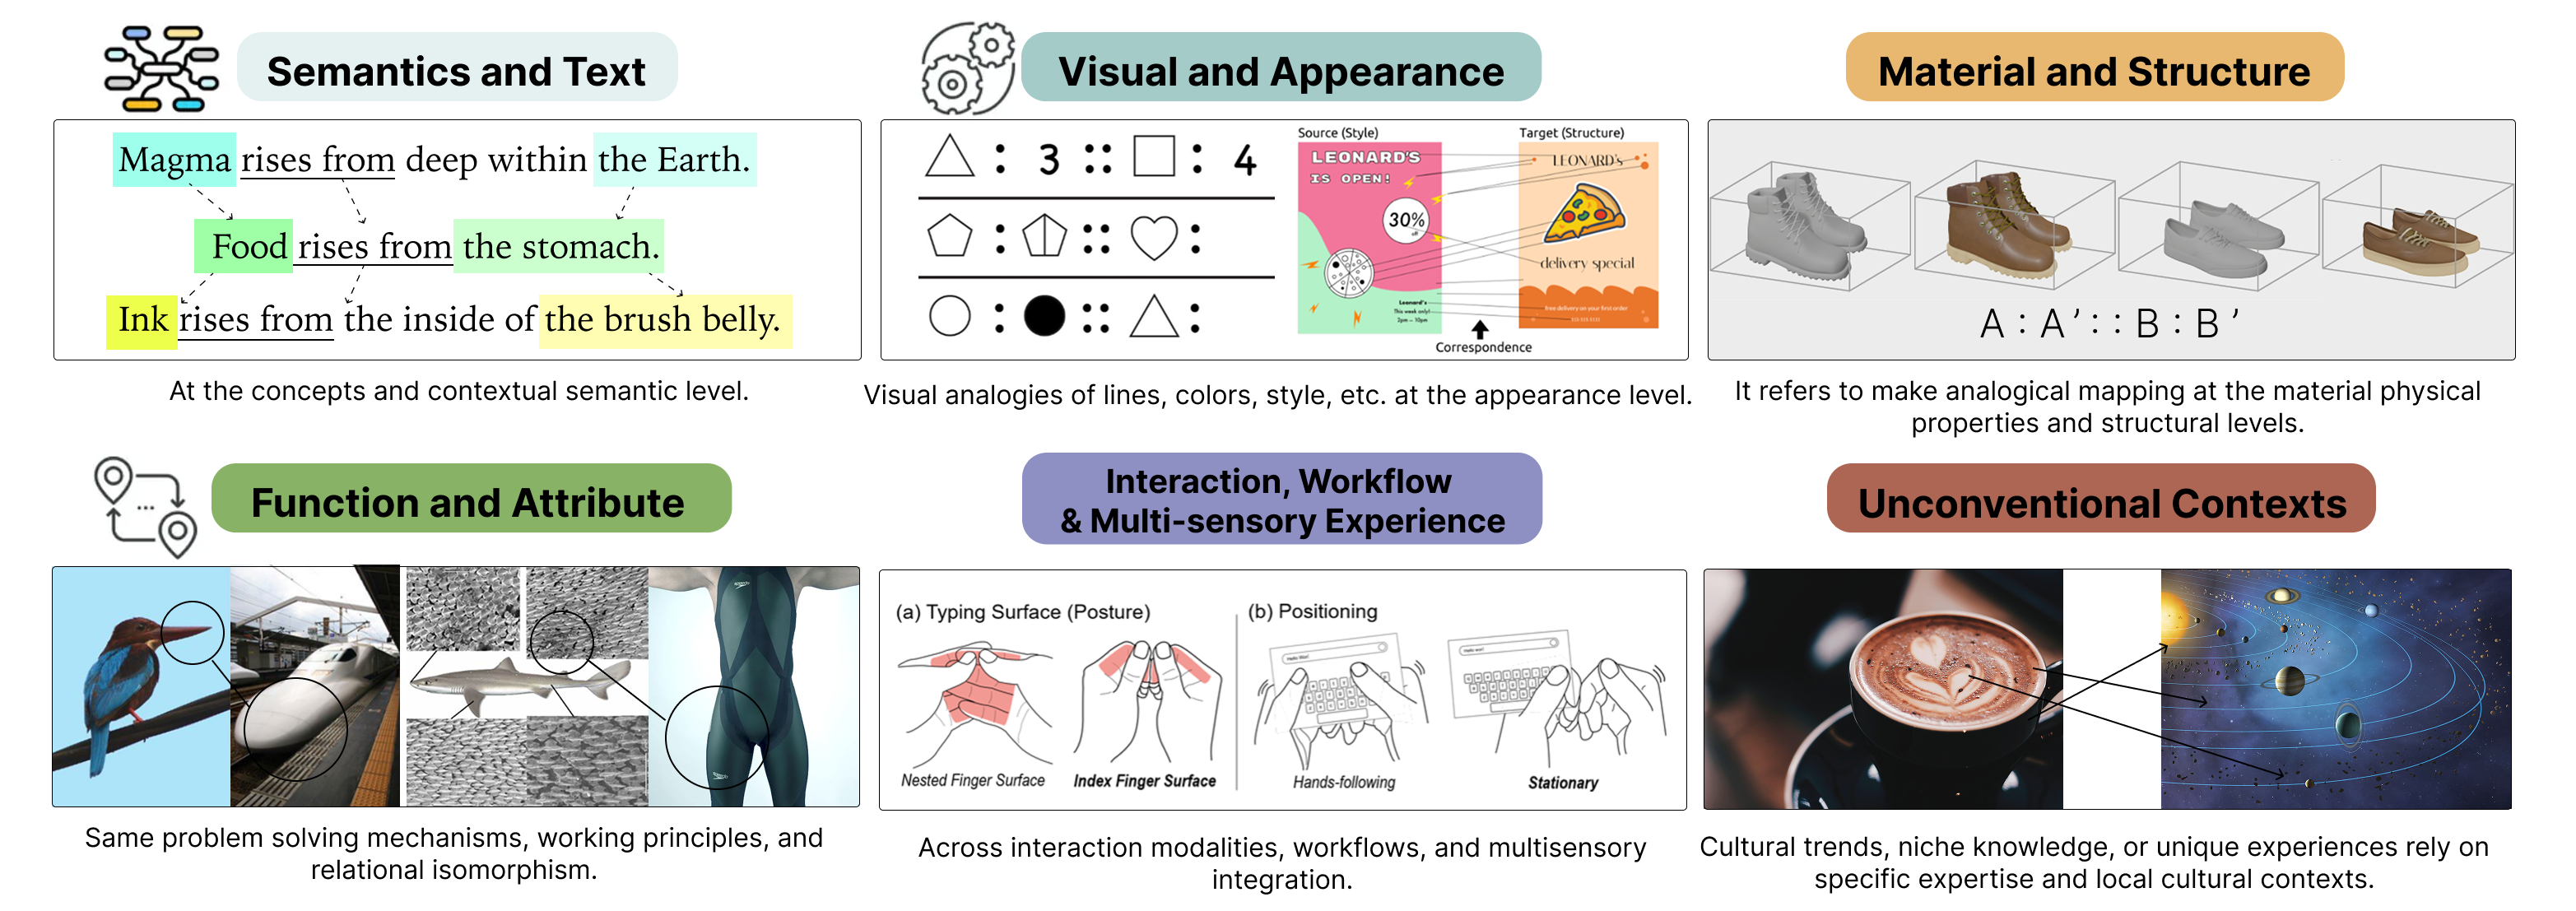
\includegraphics[width=1\linewidth]{Figures/representation.png}
    \caption{Enter Caption}
    \label{fig:Representation}
\end{figure}